\chapter{Implementazione}

\section{Onion V3}

La terza generazione di onion nasce per risolvere alcuni problemi di sicurezza. In particolare rispetto alla seconda generazione
\begin{itemize}
    \item Vengono aggiornati i sistemi di crittografia, da SHA1/DH/RSA1024 a SHA3/ed25519/curve25519
    \item Vengono migliorati i directory server e il directory protocol
    \item Viene cambiato il sistema di hostname
\end{itemize}
Precedentemente venivano usati i primi 80 bit dell'hash (SHA1) della chiave pubblica per creare un'hostname, un esempio yyhws9optuwiwsns.onion, nella terza generazione vengono codificati in base32
\begin{itemize}
    \item La chiave pubblica, un totale di 32 byte in ed25519
    \item Il checksum di 2 byte
    \item Un byte di versione, di default '\textbackslash x03' 
\end{itemize}
In totale il nuovo hostname possiede 56 caratteri \cite{Torv3} \\
Un esempio è l'indirizzo \emph{pg6mmjiyjmcrsslvykfwnntlaru7p5svn6y2ymmju6nubxndf4pscryd.onion}, una volta decriptato sfruttando il base32 definito nell' RFC 3548 e 4648 abbiamo la seguente stringa 79bcc625184b05194975c28b66b66b0469f7f6556fb1ac3189a79b40dda32f1f214703, come notiamo termina con 03, il byte di versione

\section{Studio delle tecnologie}

Per creare un servizio sulla rete onion si possono usare una moltitudine di tecnologie differenti, ogni singolo aspetto necessita di effettuare delle scelte. \\
\begin{itemize}
    \item Deploy del Server, la prima scelta ricade sulla creazione del server e in particolare scegliere dove eseguire il deploy, ci sono molteplici motivi per usare un servizio cloud, tra cui la sicurezza e la facilità d'uso. Ci sono 3 principali competitor e molti altri secondari che per la maggior parte sfruttano i server di queste 3 aziende
    \begin{itemize}
        \item Microsoft Azure
        \item Google Cloud
        \item Amazon Web Service, il più importante servizio cloud, è gestito e reso disponibile da Amazon e possiede molti servizi tra cui scegliere. Per questa implementazione useremo il servizio EC2 messo a disposizione da AWS in una macchina t3.micro
    \end{itemize}
    \item SO, la seconda scelta ricade sul sistema operativo della nostra macchina. Debian in particolare ha molti vantaggi, tra cui 
    \begin{itemize}
        \item Leggerezza, affidabilità e sicurezza derivate da un sistema GNU/Linux
        \item Maggiore utilizzo in ambienti server
        \item Nessun costo aggiuntivo derivato dall'aquisto di una licenza d'uso come Windows server
    \end{itemize}
    Useremo in particolare la versione 11
    \item Web Server, abbiamo due web server principali 
    \begin{itemize}
        \item Apache httpd, il più vecchio dei due, rilasciato con licenza Apache 2.0
        \item Nginx, un web server più moderno che fornisce diversi altri strumenti oltre al web server, tra cui il proxy e load balancer, è gratuito e come httpd è open source, ha superato apache da un paio di anni. Viene anche utilizzato in container docker, ma noi lo useremo in una classica macchina virtuale.
    \end{itemize}
\end{itemize}




\section{Creazione del servizio}

Per questa implementazione verrà usato il servizio di macchina virtuale (EC2) con Debian 11 messo da Amazon Web Service tramite il web server nginx \\
Il primissimo passo fondamentale è aggiungere alla macchina i giusti security group, altrimenti la connessione non sarebbe possibile


\begin{itemize}
    \item Consentire la connessione ssh alla porta 22
    \begin{figure}[h]
        \centering
        
\includegraphics[width=\textwidth]{securityGroup1}
        \caption{security Group 1, ssh in entrata}
        \label{fig:sec1}
    \end{figure}
    
    \item Consentire il traffico TCP in uscita
    \begin{figure}[h]
        \centering
        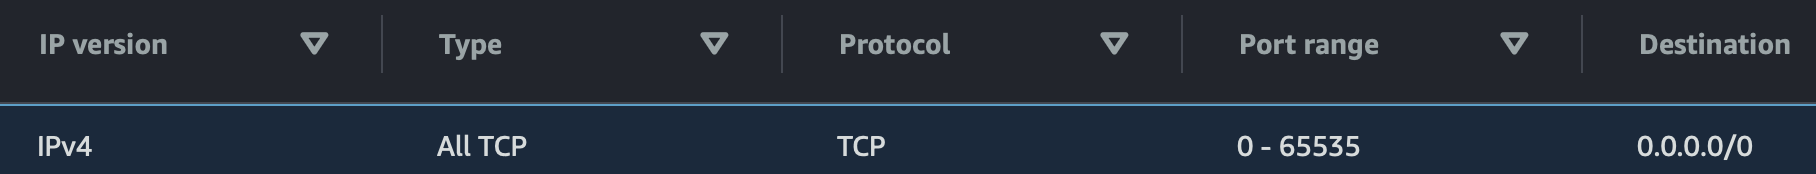
\includegraphics[width=\textwidth]{securityGroup2}
        \caption{security Group 2, TCP in uscita}
        \label{fig:sec2}
    \end{figure}
\end{itemize}

È inoltre importante creare una coppia chiave pubblica/privata, useremo la chiave privata con formato *.pem per tentare la connessione
% [caption=connessione ssh]
% \lstinline{}
\begin{lstlisting}
    ssh -i key.pem admin@*.compute.amazonaws.com
\end{lstlisting}

La primissima operazione sarà l'aggiornamento dei repository e successivamente del sistema
% [caption=aggiornamento sistema]
\begin{lstlisting}
    sudo apt update && sudo apt full-upgrade -y
\end{lstlisting}

Poi installiamo il web server
%[caption=Installazione Nginx]
\begin{lstlisting}
    sudo apt install nginx
\end{lstlisting}

Una volta completata l'installazione il web server è già avviato e in ascolto sulla porta 80

\section{Tor \& unix socket}
Per configurare tor è innanzitutto necessario aggiungere il repository, installiamo \textbf{apt-transport-https} per utilizzare i repository tramite https
\begin{lstlisting}
    sudo apt install apt-transport-https
\end{lstlisting}
Poi aggiungiamo i repository nella cartella \lstinline{/etc/apt/sources.list.d} \\
Dal comando \lstinline{lsb_release -c} possiamo vedere la distribuzione corrente e inserirla nella configurazione, in questo caso bullseye è la nostra distribuzione, inseriamo nel file tor.list i seguenti 
\begin{lstlisting}
    deb [signed-by=/usr/share/keyrings/tor-archive-keyring.gpg] https://deb.torproject.org/torproject.org bullseye main
    deb-src [signed-by=/usr/share/keyrings/tor-archive-keyring.gpg] https://deb.torproject.org/torproject.org bullseye main
\end{lstlisting}
Aggiungiamo le chiavi gpg della repository appena aggiunta
\begin{lstlisting}
    wget -qO- https://deb.torproject.org/torproject.org/A3C4F0F979CAA22CDBA8F512EE8CBC9E886DDD89.asc | gpg --dearmor | tee /usr/share/keyrings/tor-archive-keyring.gpg >/dev/null
\end{lstlisting}
Assicuriamoci inoltre che gpg sia installato nel sistema
\begin{lstlisting}
    sudo apt install gpg
\end{lstlisting}
Aggiorniamo gli index ed installiamo finalmente tor
\begin{lstlisting}
    sudo apt update && sudo apt install tor -y 
\end{lstlisting} \cite{TorRepo}
Generiamo il torrc file che ci servirà per impostare tutti i parametri di configurazione 
\begin{lstlisting}
    sudo tor -f /etc/tor/torrc
\end{lstlisting}
Apriamo il file e togliamo il commento alle righe \lstinline{HiddenServicePort 80 127.0.0.1:80} e \lstinline{HiddenServiceDir *}, il primo ci serve per indicare la directory in cui si trovano le informazioni del sito e le chiavi crittografiche, il secondo indica che il traffico arrivato dalla porta virtuale (80), che gli utenti onion useranno per la connessione, viene reindirizzato alla porta 80 del localhost, ovvero la porta in cui è in ascolto il web server nginx. \\
Riavviamo tor per assicurarci che il file di configurazione torrc non abbia errori
\begin{lstlisting}
    sudo systemctl restart tor
\end{lstlisting}
A questo punto tor ha creato gli introduction points e ha generato un circuito con ognuno di essi, ha generato le chiavi ed il proprio hostname, queste informazioni sono state aggiunte nella cartella che abbiamo inserito nell'HiddenServicePort, in particolare hostname contiene l'indirizzo tor del nostro servizio \cite{SetupOnionService} \\
Questo sistema però non è completamente sicuro, stiamo collegando tor con il web server tramite una porta, essendo entrambi i processi sulla stessa macchina il sistema ottimale è utilizzare un socket unix tra i due processi. Questo impedisce ad un utente non Tor di accedere direttamente al web server senza dover configurare firewall che comunque aggiungono complessità nella rete \\
Apriamo il file \lstinline{/etc/nginx/sites-enabled/default} e nella sezione server aggiungiamo il socket in ascolto, cosi che la comunicazione possa passare anche per il socket unix
\begin{lstlisting}
    listen unix:/var/run/website.sock;
\end{lstlisting}
Possiamo inoltre rimuovere la connessione dalla porta 80 commentando le seguenti righe
\begin{lstlisting}
    #listen 80 default_server;
    #listen [::]:80 default_server;
\end{lstlisting}
Dopo aver riavviato nginx ed esserci assicurati che non vi siano errori apriamo il file torrc e inseriamo lo stesso socket
\begin{lstlisting}
    HiddenServicePort 80 unix:/var/run/website.sock
\end{lstlisting}
Infine riavviamo tor, se tutto è andato a buon fine il servizio dovrebbe essere in grado di rispondere
\begin{lstlisting}
    sudo systemctl restart tor
\end{lstlisting}

\importImage{
    \label{fig:nginxConnection} 
    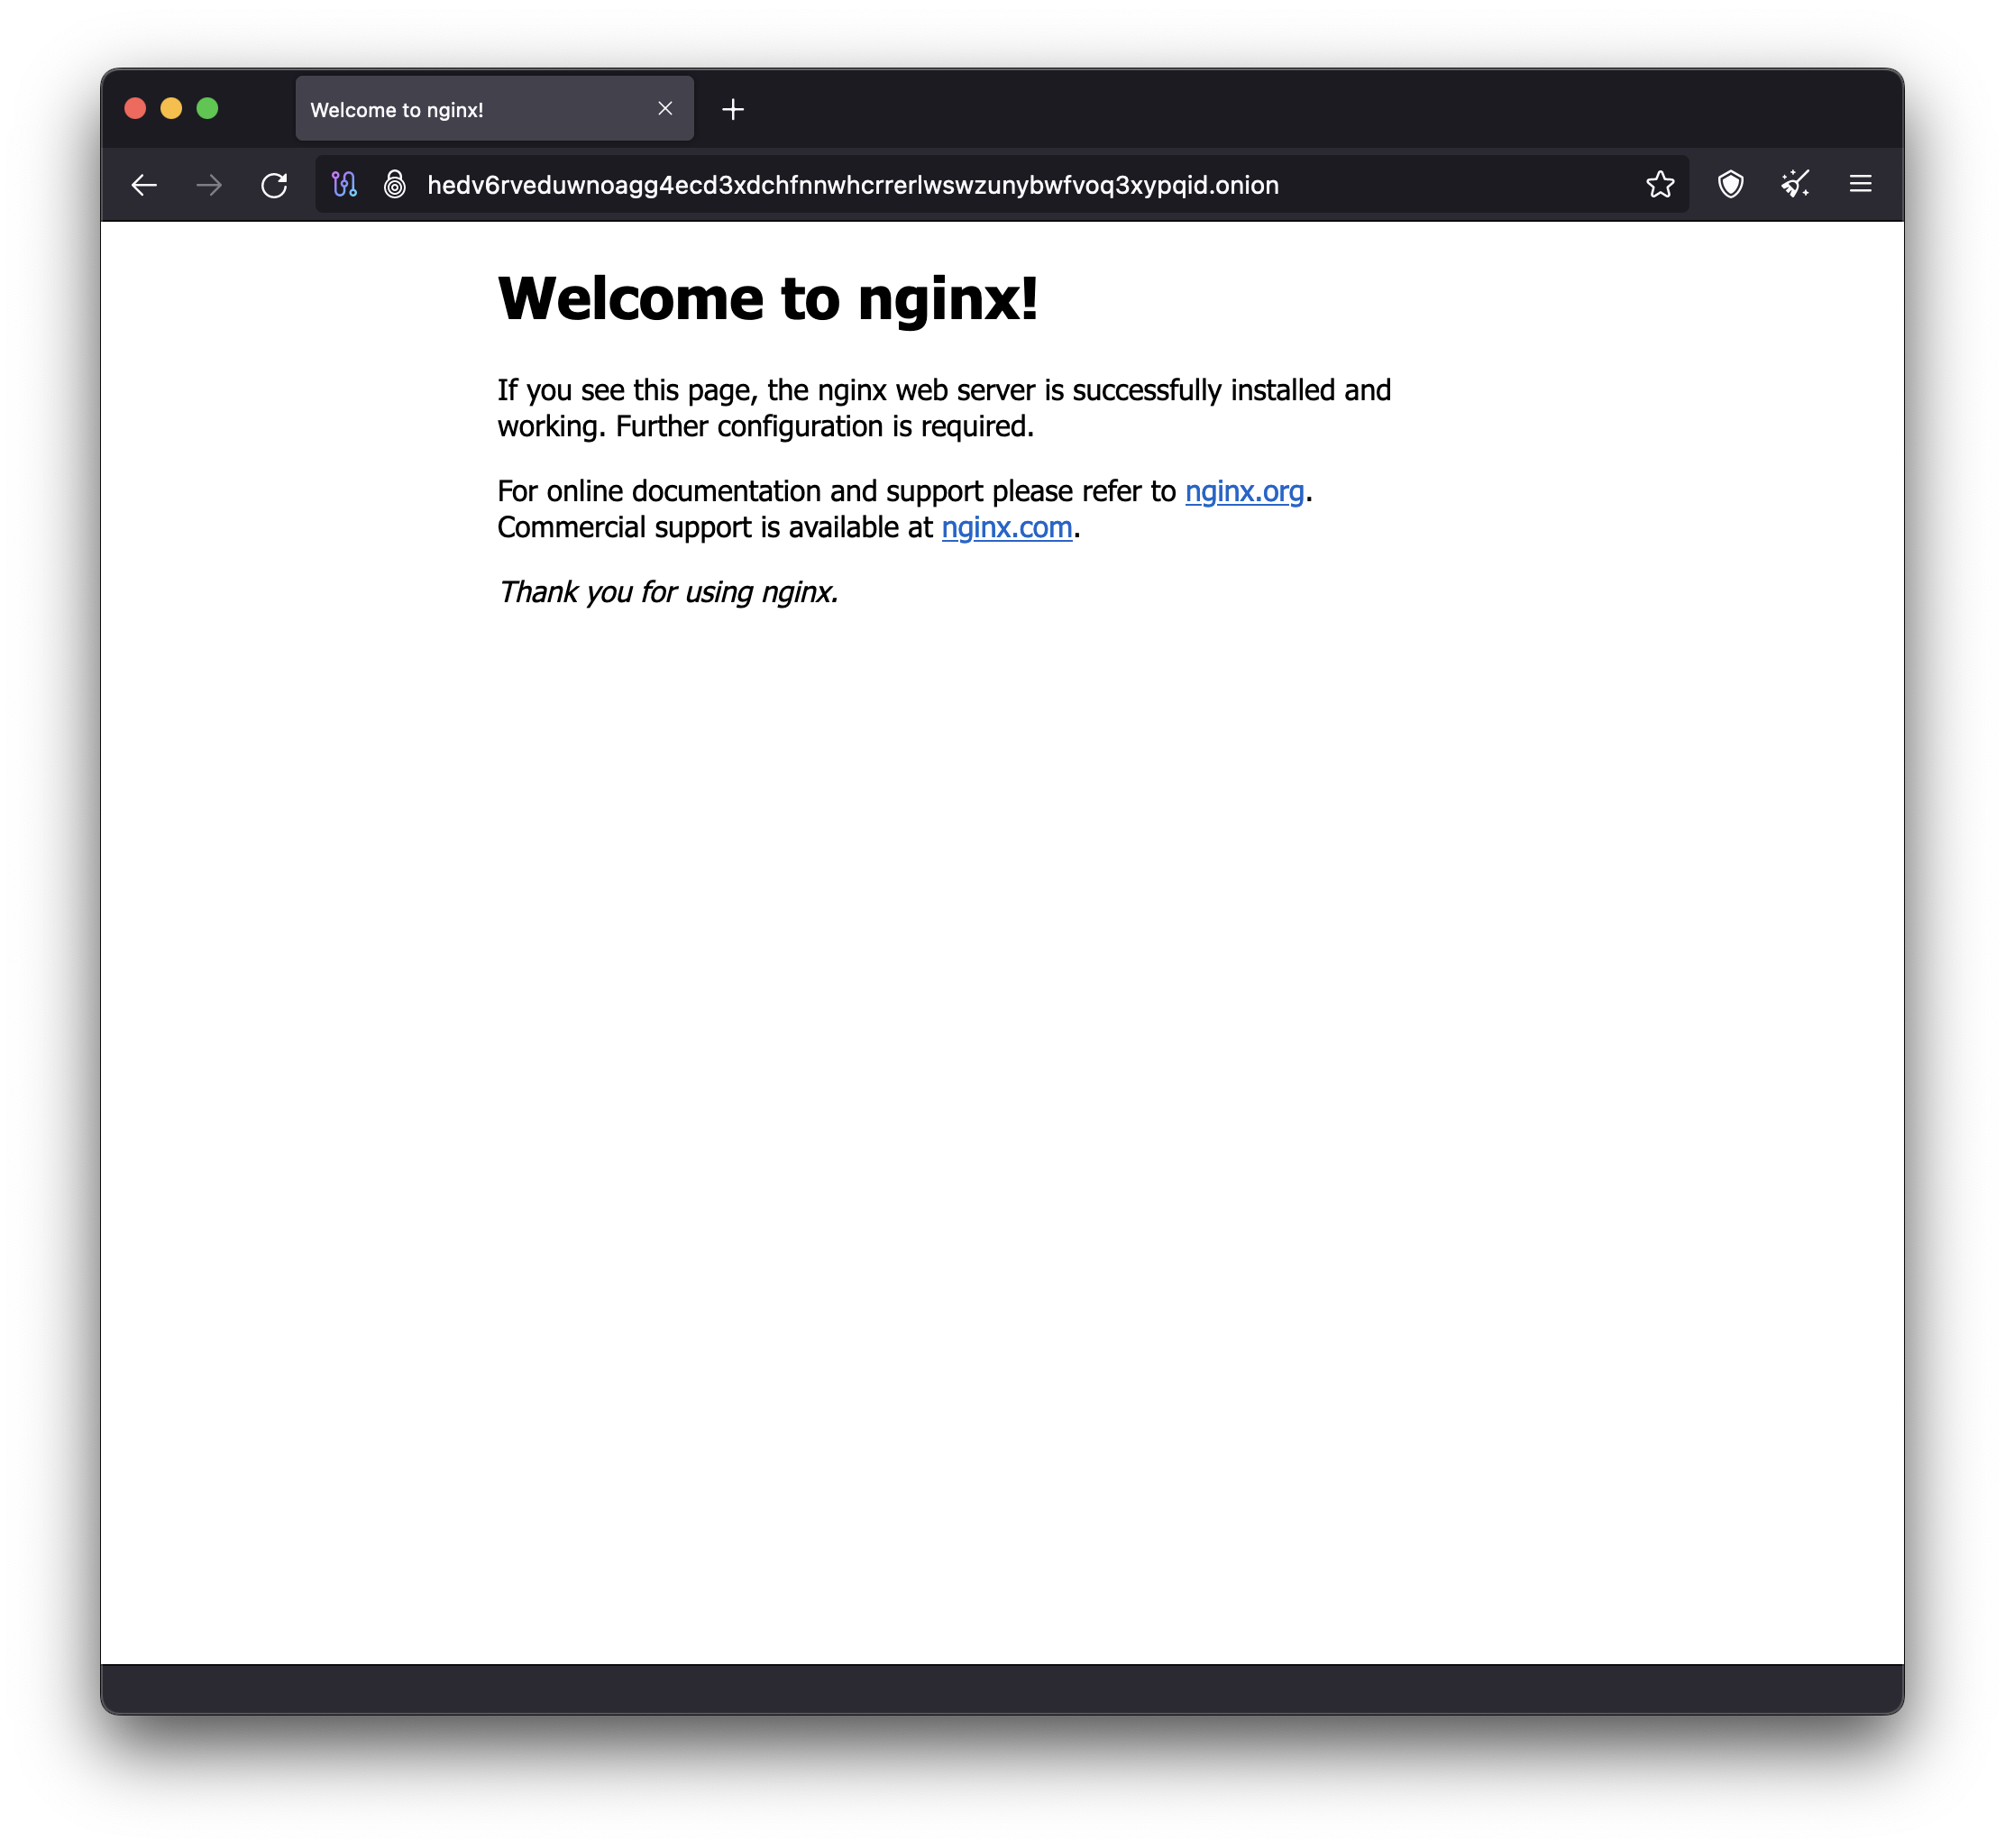
\includegraphics[width=\textwidth]{connectionSucceeded}
    \caption{Connessione al web server nginx}
}
